% Author: Elena Marochkina <xmaroc00@stud.fit.vutbr.cz>
% Author: Nikita Pasynkov <xpasyn00@stud.fit.vutbr.cz>

\documentclass[12pt, a4paper]{article}

\usepackage[czech]{babel}
\usepackage[utf8]{inputenc}
\usepackage[T1]{fontenc}
\usepackage[left=2cm, top=3cm, text={17cm, 24cm}]{geometry}
\usepackage{times}
\usepackage{graphicx}
\usepackage{pdflscape}

\begin{document}
\begin{titlepage}
\begin{center}
    \includegraphics[width=0.77 \linewidth]{FIT_logo.pdf} \\
    \vspace{\stretch{0.382}}
    \Huge{Projekt 1.~část} \\
    \Huge{Datový model (ERD) a model případů užití} \\
    \Large{\textbf{Zadání č.~40.\,--\, Internetový obchod}} \\
    \Large{Databázové systémy}
    \vspace{\stretch{0.618}}
\end{center}

{\Large
    \today
    \hfill
    \begin{tabular}{l l}
		Nikita Pasynkov & (xpasyn00) \\
		Elena Marochkina & (xmaroc00) \\
    \end{tabular}
}
\end{titlepage}

% Obsah %
\pagenumbering{roman}
\setcounter{page}{1}
\tableofcontents
\clearpage

% Zadání %
\pagenumbering{arabic}
\setcounter{page}{1}

\section{Zadání}
Cílem je vytvoření jednoduché aplikace pro internetový obchod s určitým druhem zboží např. knihkupectví. Návštěvníci WWW stránek mají možnost prohlížet si veškerý sortiment obchodu, který je členěn do kategorií, ať už daný produkt je skladem či nikoliv. Pokud má návštěvník zájem o určitý produkt, může si jej vybrat (vložení do nákupního košíku). Vybrané zboží si může objednat po zadání potřebných údajů (kontakt, doprava, ...). Zboží si může objednat pouze registrovaný uživatel, pokud uživatel nakupuje poprvé, musí se zaregistrovat a získá přihlašovací jméno a heslo. Tyto údaje může použit k modifikaci osobních informací. Po zaplacení zákazníkem za zboží je považována obchodní transakce za vyřízenou a zaměstnanec obchodu vyexpeduje zboží podle objednávky. Vedení obchodu má informace o celkových tržbách, oblíbenosti zboží, jeho kapacitě, o objednávkách, kdo ji vyřizoval atd.
% Datový model (ERD) %
\newpage

\section{Datový model (ERD)}
\subsection{Popis ERD}

V internetovém obchodě jsou dva typy uživatelů: registrované uživatele a zaměstnancí. Protože se jedná o podskupiny s různými atributy, rozhodli jsme se použít specializaci.

O uživatelích uchováváme tyto informace: jméno a příjmení, přihlašovací jméno, heslo, adresa, telefon, e-mail.

Uživatel může vkládat zboží do košíku (vztah k entitě Košík). Nákupní košík obsahuje zboží z internetového obchodu. Jako atributy zboží ukládáme následující informace: název, cena, počet zboží. Každé zboží je členěno do kategorií (vztah k entitě Kategorie).

Číslo košíku zůstane pro každého uživatele stejné až do provedení objednávky, po zadání objednávky se číslo košíku změní.

Následně může uživatel  tvořit objednávku z košíku (vztah k entitě Objednavka). Každá objednávka má atribut stav, který může nabývat následujících hodnot: vytvořeno, zaplaceno, expedovano, zrušeno. 

Dokud uživatel neprovede platbu za zboží (vztah k entitě Platba), nemůže mít objednávka stav zaplaceno. Uživatel může objednávku zrušit sám nebo pokud uživatel neuhradí objednávku do 7 dnů, stav objednávky se automaticky změní na zrušeno.

Platbu provádí uživatel pouze online. Částka platby bude porovnána s požadovanou částkou platby za objednávku (výpočet počtu položek v košíku s jejich cenou).

Každá objednávka po zaplacení je přidělena zaměstnanci, který ji expeduje (vztah k entitě Zaměstnanec) podle obsahu košíku.
Informace o zaměstnancích taky ukládáme do našeho systému. Zaměstnance máme ve svém IS pouze z toho důvodu, aby bylo možné zjistit, který zaměstnanec objednávku vyzvedl a odeslal a pro tyto účely uchováváme pouze základní informace o zaměstnancích.

 \begin{landscape}
 \begin{figure}[!ht]
    \centering
    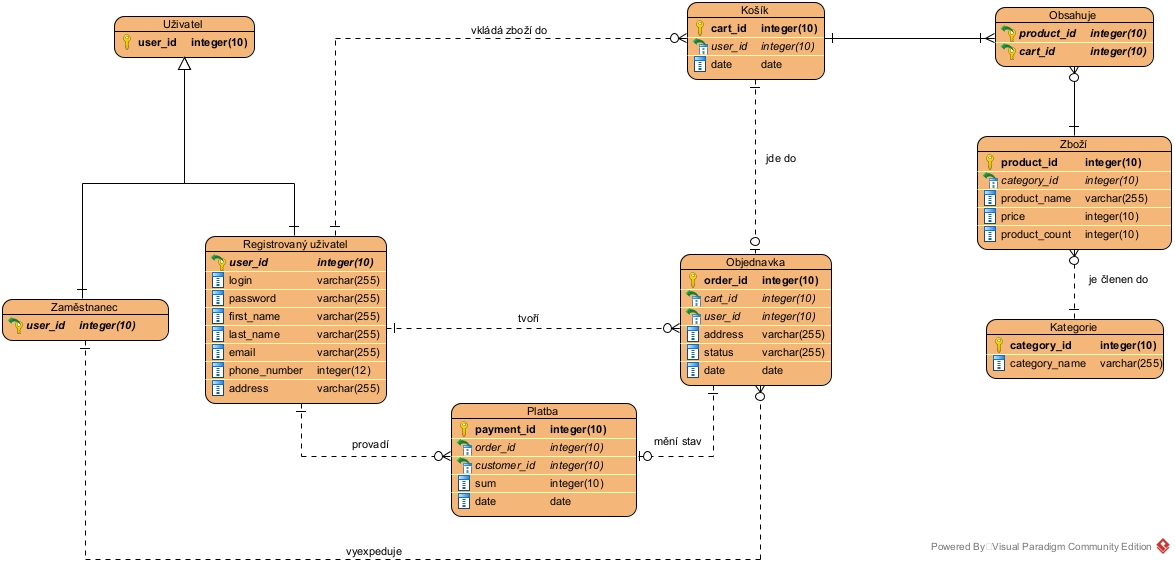
\includegraphics[width=1\linewidth]{IDS_ER_diagram.jpg}
    \caption{Datový model (ERD)}
    \label{figure:ast_example1}
\end{figure}

\end{landscape}

% Datový model (ERD) %
\newpage
\section{Model případů užití}


 \begin{figure}[!ht]
    \centering
    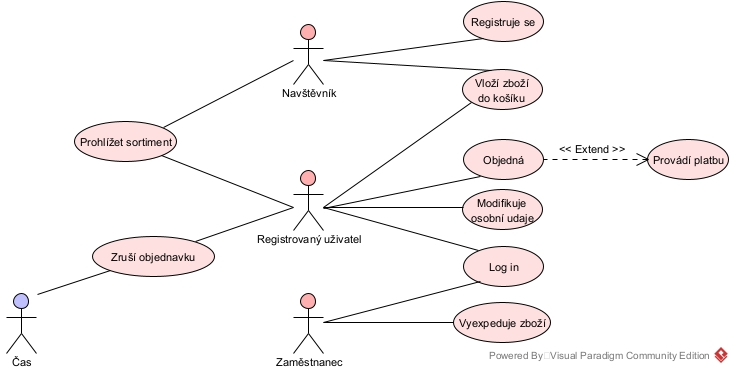
\includegraphics[width=1\linewidth]{use_case_diagram.jpg}
    \caption{Model případů užití}
    \label{figure:ast_example1}
\end{figure}
\end{document}
